\begin{figure}[H]
  \centering
  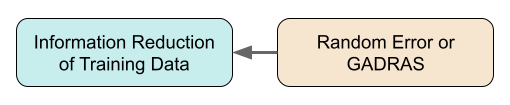
\includegraphics[width=0.7\linewidth]{./chapters/method/methodology2.png}
  \caption{Second portion of the flowchart from Figure \ref{fig:method} being 
           described in this section.}
\end{figure}

The overall goal of this project is to determine how much information to what
quality is needed to train an \gls{ML} model that can provide \gls{SNF}
attribution by correctly predicting the reactor type, burnup, \gls{U235}
enrichment, and time since irradiation.  In this section, the process of
information reduction of the training database is outlined for each experiment. 

The first experiment introduces the nuclide masses to a uniform uncertainty via
random error, and the second experiment computes a gamma spectrum for each
sample in the database from the nuclide activities in Section
\ref{sec:snffeats}.  This detector-based treatment is not being applied to the
mass measurements because studying measurement techniques that can only be done
in a lab is not the goal of this work.  Instead, field-deployable detectors are
of interest. \todo[inline]{make sure this is mentioned in the intro}

\subsection{1$^{\mathbf{st}}$ Experiment: Nuclide Masses}
\label{sec:masserr}

The training database for the first experiment is meant to be a proof of
principle with the developed methodology, and mimic a scenario where there is
"perfect knowledge" of a set of nuclides of interest. It is still interesting,
however, to probe how the statistical models perform under increasing error in
the nuclide measurements. Therefore error and uncertainty were injected into
the nuclide mass measurements in the training database for the machine learning
algorithms and \gls{MLL} calculations, respectively. 

\noindent \textbf{Machine Learning Algorithms} : For the \textit{k}-nearest
neighbor and decision tree algorithms, a uniform error is applied randomly to
each nuclide mass as follows.  For a maximum error $E_{max}$ between the values
of $0.0 < E_{max} < 0.2$, each nuclide mass is peturbed by a random fraction in
the range: $[1-E_{max},1+E_{max}]$.  Therefore the $0\%$ error case represents
full knowledge of nuclide masses, and that knowledge slowly decreases up to
$20\%$. 

\noindent \textbf{Maximum Likelihood Calculations} : For the \gls{MLL}
calculations, a uniform uncertainty was introduced to each nuclide mass.  Thus,
each nuclide is given an uncertainty of $5\%$, $10\%$, $15\%$, and $20\%$
via:
\begin{equation}
  \label{eq:mllunc}
  \sigma_{Log L}^2 = \sum_j \left( 
                            \frac{r_{j,test} - r_{j,sim}}{\sigma_{j,sim}^2}
                            \right)^2 
                            (\sigma_{j,sim}^2 + \sigma_{j,test}^2)
\end{equation}
where $r_{j,sim}$ and $r_{j,test}$ are the nuclide measurements for the
simulated/training set samples and the test samples, respectively, and
$\sigma_{j,sim}$ and $\sigma_{j,test}$ are their respective standard
deviations calculated from the four uncertainty levels listed above.

\subsection{2$^{\mathbf{nd}}$ Experiment: Gamma Spectra}
\label{sec:gamerr}

Moving beyond injecting uniform error to a nuclide mass measurement, the next
step in information reduction takes place for the second experiment, which uses
processed gamma spectra for the training database.  The code \gls{GADRAS}
\cite{gadras} developed at Sandia National Laboratories will provide
computational gamma spectra.  This adds more than one layer of reduced
information quality, which are listed here as an outline of the steps taken to
process the gamma spectra:

\begin{enumerate}
  \item \label{itm:1} The list of nuclides is limited to radionuclides.
  \item \label{itm:2} Instead of "perfect" radionuclide activity knowledge, 
        they are being measured by a gamma detector.
  \item \label{itm:3} The processing of the gamma spectra can be highly variable.
  \item \label{itm:4} The $\sqrt{n}$ error of counts-based detection is included. 
\end{enumerate}

Step \ref{itm:1} covers which radionuclides to include, which was previously
covered in Section \ref{sec:snffeats}. Step \ref{itm:2} is to obtain a gamma
spectrum for every \gls{SNF} entry in the database. This is done using the
\gls{GADRAS} tool, which applies a \gls{DRF} to the gamma lines from these
radionuclides. The input is a nuclide activity vector, and the output is an
array of energy bins (measured in $keV$), and the counts per energy bin.

The nuclide activity data did require some processing to be used in this way.
The activities that come from the \gls{ORIGEN} simulations are based on there
being $1\:MT$ of initial uranium-based fuel. Not only is this quantity an
unlikely amount to be smuggled, it would overwhelm a detector at the
\todo[inline]{fix this to be better technical explanation of dead time and pile
up} source-detector distances in \gls{GADRAS}. Therefore, the material (and
resulting nuclide activities) are scaled to be $1\:g$ of \gls{SNF}.

Regarding the input information for the \gls{GADRAS} calculations, the sources
are provided without any background; this is because any spectrum would undergo
background subtraction before further analysis. Additionally, the nuclides are
pre-decayed in \gls{ORIGEN} to correspond to various cooling times, but the
source age provided to \gls{GADRAS} needs to be a non-zero value. A source age
of $20\:minutes$ provides the expected peaks.

\begin{table}[!htb]
  \centering
  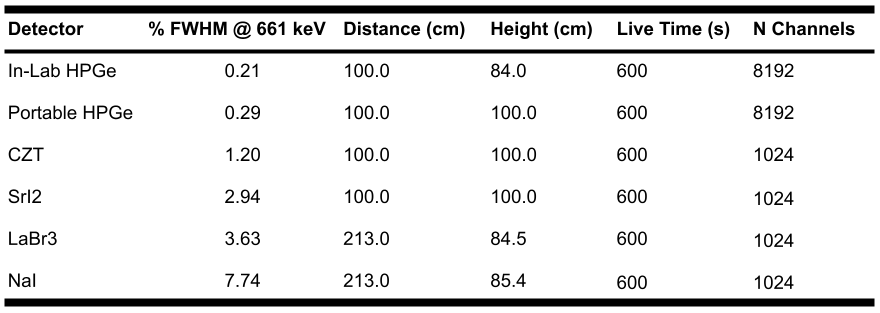
\includegraphics[width=\linewidth]{./chapters/method/gadras_detectors.png}
  \caption{Select details of 6 detector setups used to obtain gamma 
           spectra-based training databases.}
  \label{tbl:detsetups}
\todo[inline]{update this table if live times for nai and labr3 change}
\end{table}

Training databases were created for the six detectors outlined in Table
\ref{tbl:detsetups}. They were chosen to compare the highest energy resolution
detector, a lab-based \gls{HPGe}, against the rest, in order of decreasing
energy resolution: portable \gls{HPGe}, \gls{CZT}, \gls{SrI2}, \gls{LaBr3}, and
\gls{NaI} detectors. This is displayed in the table by including the \gls{FWHM}
of the $661\:keV$ peak for Cs137. At this point, there are six versions of the
original database for each detector setup, but there is a full gamma spectrum
for each \gls{SNF} entry. It is not computationally prudent to use full gamma
spectra for training and testing, and so these spectra are processed; this is
step \ref{itm:3} from above, and is outlined as follows.

\begin{figure}[!htb]
  \makebox[\textwidth][c]{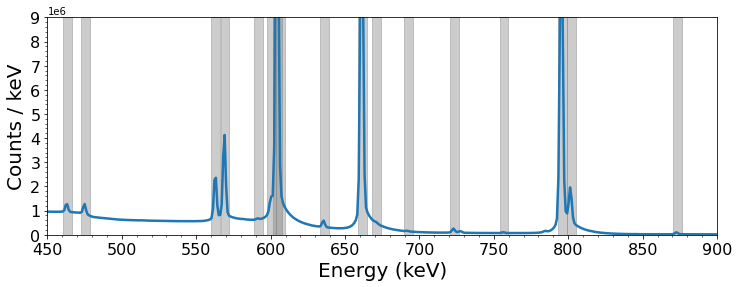
\includegraphics[width=\linewidth]{./chapters/method/energy_window_example.png}}
  \caption{Slice of an example gamma spectrum in one of the training databases
           showing the windows over the gamma energy peaks.}
  \todo[inline]{update?}
  \label{fig:enwindows}
\end{figure}

Explanation of Step \ref{itm:3} here. 

\begin{table}[!htb]
  \centering
  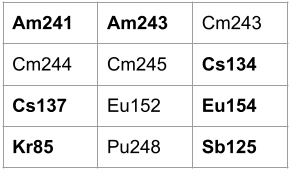
\includegraphics[width=0.4\linewidth]{./chapters/method/enlist_nucs.png}
  \caption{Nuclides that are represented by the gamma energy lines in the two . The entire 
           set of 11 nuclides belongs to the long list, and the 6 bold nuclides
           belong to the short list.}
  \label{tbl:enlistnucs}
\todo[inline]{placeholder list, update me.}
\end{table}

Lastly, step \ref{itm:4} involves the inclusion of the counting error for the
summed energy windows. This is quite simple, as statistical counting error of
$n$ counts is $\sqrt{n}$.  As in Section \ref{sec:masserr}, this error gets
applied in the same way for the machine learning algorithms, where the uniform
error is applied randomly within the range $[r-\sqrt{r},r+\sqrt{r}]$ for each
summed energy window $r$. For the \gls{MLL} calculations, Equation
\ref{eq:mllunc} is used, where $\sigma_{j} = \sqrt{r}$.  \todo[inline]{make
sure variables are explained clearly, choosing r to match variables above, the
original variable choice comes from TAMU papers}
